\documentclass[a4paper,landscape]{slides}
\usepackage{geometry}
\geometry{a4paper,total={257mm,170mm},left=20mm,top=20mm}
%
%----------------------------------------------------------
% This is a sample document for the LaTeX Slides Class
% Class options
%       --  Body text point size (normalsize) is 27 (default)
%           and can not be adjusted to any other value.
%       --  Paper size:  letterpaper (8.5x11 inch, default)
%                        a4paper, a5paper, b5paper,
%                        legalpaper, executivepaper
%       --  Orientation (portrait is the default):
%                        landscape
%       --  Quality:     final(default), draft
%       --  Title page:  titlepage, notitlepage
%       --  Columns:     onecolumn (default), [twocolumn is not avalible]
%       --  Equation numbering (equation numbers on the right is the default)
%                        leqno (equation numbers on the left)
%       --  Displayed equations (centered is the default)
%                    fleqn (flush left)
%
%  \documentclass[a4papr,fleqn]{slides}
%
%  The slides are separated from each other by the slide
%  environment, see below:
%
\usepackage{graphicx}
\graphicspath{ {images/} }

%------------------------------------------------------------------

\begin{document}

% ----------------------------------------------------------------
% PAGE TITLE
% ----------------------------------------------------------------
\title{\Huge \bfseries Data Analysis: \\ Programming}
\author{\vspace{1cm} Institute of Technology Tallaght}
\date{Department of Computing}
\maketitle
\newpage



% ----------------------------------------------------------------
% PAGE R INTRO
% ---------------------------------------------------------------2
{\Large \bfseries R}
\vspace{-1cm}
\begin{itemize}
\setlength\itemsep{-0.5em}
\item R is an interpreted programming language for data processing and visualisation
\item It incorporates many statistical methods, both simple and advanced
\item Based on the S language that was developed by researchers at Bell Labs in New Jersey
\item Developed by Ross Ihaka and Robert Gntleman at University of Auckland in New Zealand under the GNU public license (early 1980s)
\item Today, maintained by a dedicated group called the R Core Team
\end{itemize}
\newpage

{\bfseries General\\}
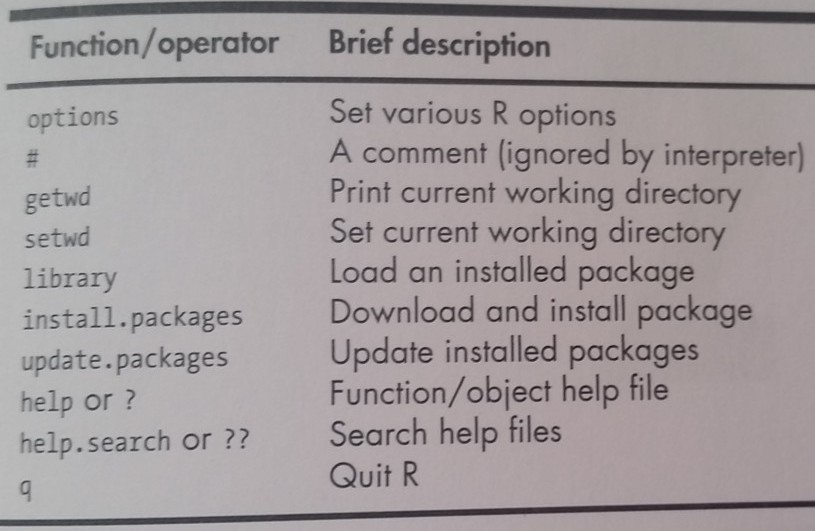
\includegraphics[width=0.5\textwidth]{ch1.jpg}
\newpage

{\bfseries Numerics, Arithmetic, Assignment and Vectors\\}
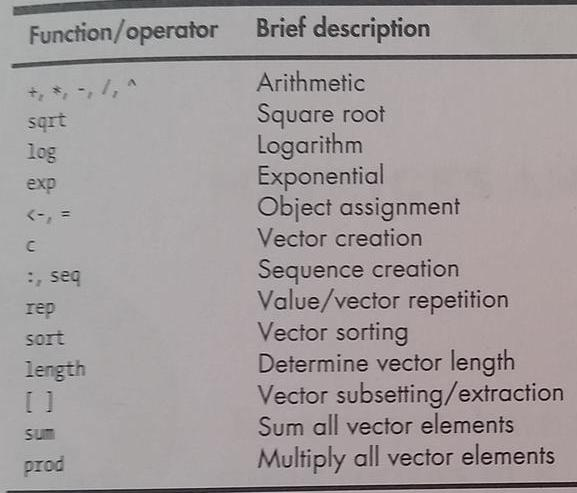
\includegraphics[width=0.5\textwidth]{ch2.jpg}
\newpage

{\bfseries Matrices and Arrays\\}
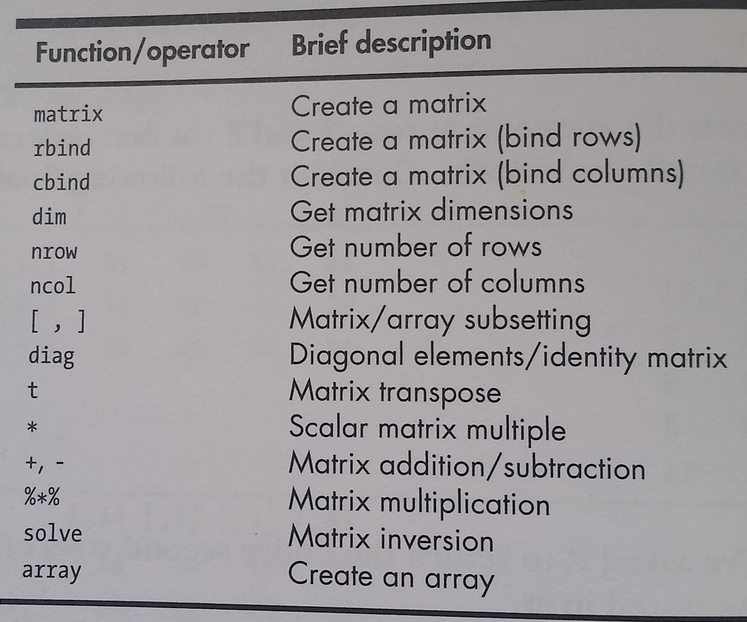
\includegraphics[width=0.5\textwidth]{ch3.jpg}
\newpage

{\bfseries Non-Numeric Values\\}
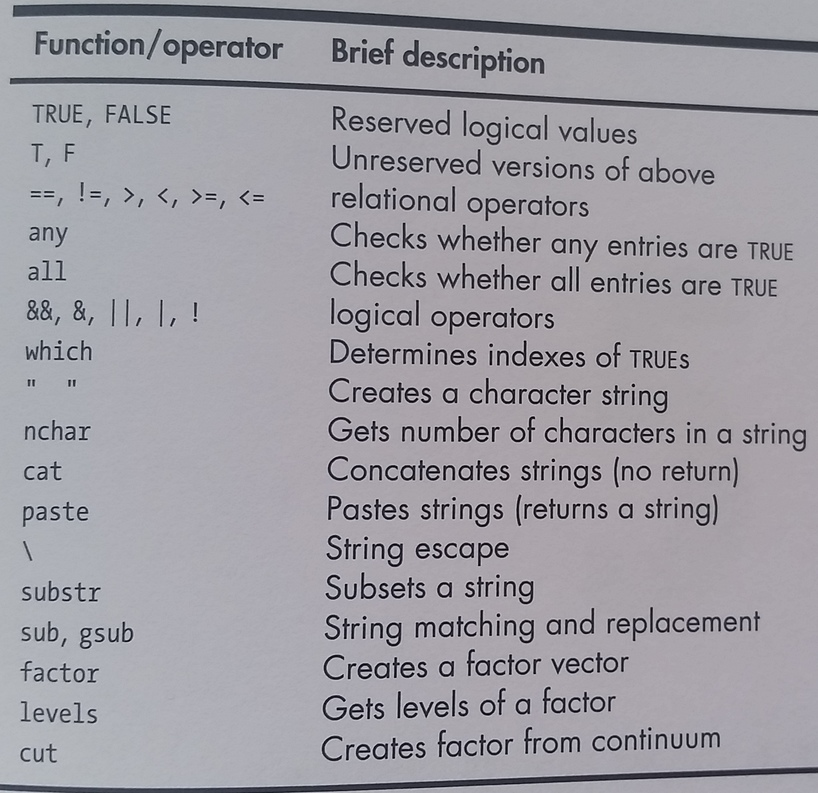
\includegraphics[width=0.5\textwidth]{ch4.jpg}
\newpage

{\bfseries Lists and Data Frames\\}
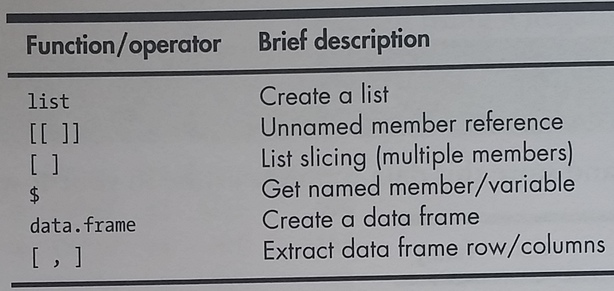
\includegraphics[width=0.5\textwidth]{ch5.jpg}
\newpage

{\bfseries Special Values, Classes and Coercion \\}
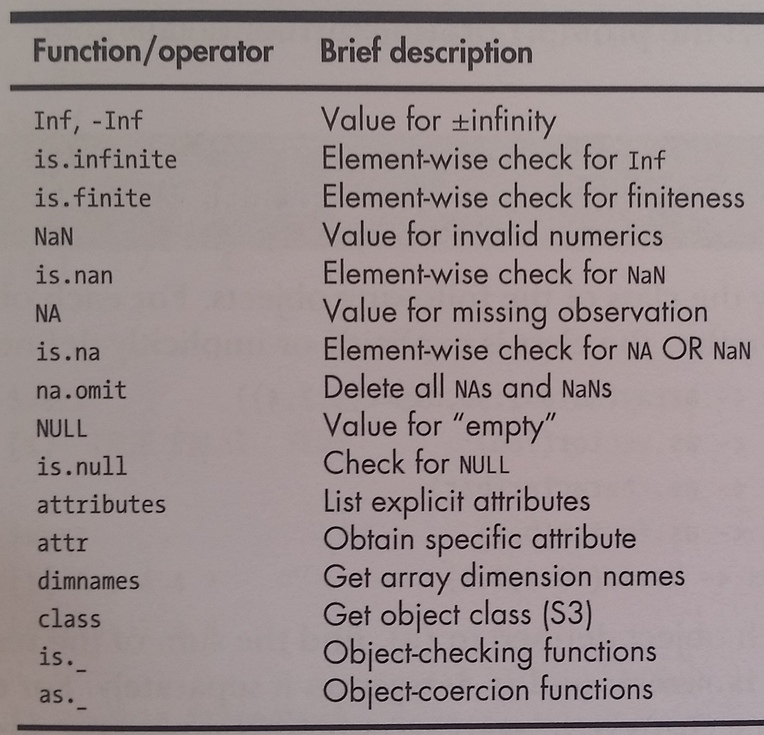
\includegraphics[width=0.5\textwidth]{ch6.jpg}
\newpage

{\bfseries Basic Plotting\\}
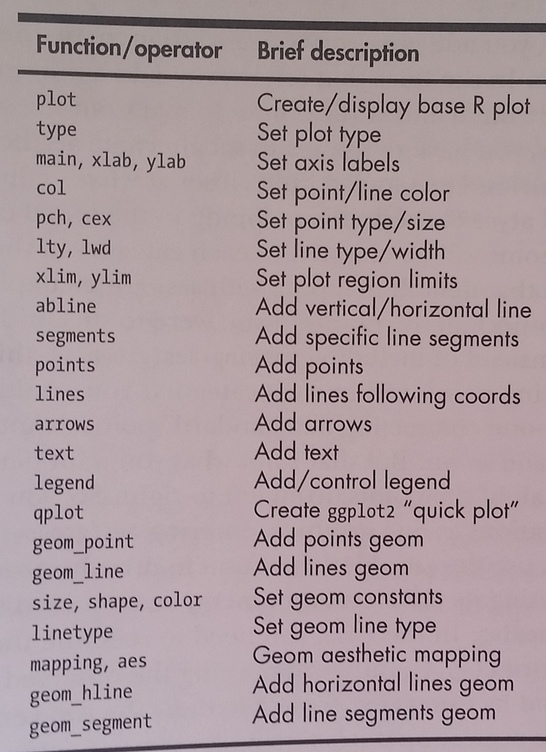
\includegraphics[width=0.4\textwidth]{ch7.jpg}
\newpage

\end{document}
